\section{Expérimentation et Résultats}\label{Expérimentation et Résultats}
Dans cette section, nous présentons les performances de notre modèle de prédiction  du paludisme à travers une analyse des résultats des expérimentations que nous avons menées sur des jeux de données du  réelles de patients  et un jeu de données semi-synthétique obtenue  à partir du jeu de données réelles. Nous commençons par présenter les conditions d’expérimentation
\subsection{Conditions d’expérimentations}
Nous avons testé le modèle sur trois jeux de données différents en implémentant l’algorithme de la régression logistique avec le logiciel Python. Pour imputer  les données manquantes, nous avons utilisé le package missForest du logiciel R est utilisé.

\subsubsection{Nos jeux de données.} Nous avons collecté et utilisé un jeu de données patient réels provenant de différents points de santé qui ont été définis lors du Grand Magal de Touba en 2016. Nous avons également généré et utilisé deux variantes de ce jeu de données de patient réels. La description des caractéristiques de notre jeu de données brutes de patients réels, ainsi que le processus  de préparation des données que nous avions proposées pour nettoyer, normaliser et imputer les informations, sont données dans la section \ref{data_prep}. Nous notons \textsc{DT1} ce jeu de données.
La première variante, notée \textsc{DT2} est obtenue en supprimant les enregistrements avec les attributs manquants dans \textsc{DT1} au lieu d'utiliser un algorithme d'imputation qui prédit les valeurs des informations manquantes.

Une telle variante aidera à étudier l’impact de la suppression des enregistrements avec des valeurs manquantes dans l'exactitude de la prévision.
La deuxième variante, appelée \textsc{DT3}, est un jeu de données semi-synthétique qui a été généré en utilisant une stratégie de sur échantillonnage sur le jeu  de données brutes \textsc{DT1}. En effet une analyse explicative effectuée sur le jeu de données \textsc{DT1} a révélé que les données sont assez déséquilibrés, c'est-à-dire qu'il montre un déséquilibre important entre les classes; le nombre de  patients atteints de paludisme était largement inférieur au nombre de patients qui ne souffrent pas de paludisme, comme illustré à la figure \ref{records_class}. L’exploitation des approches d'échantillonnage peut permettre d’obtenir un jeu de données équilibré concernant les deux classes à prédire. 
Pour cela nous avons implémenté l’algorithme SMOTE \cite{Wa06},  avec le package \emph{imbalanced-learn} \cite{Gu17}. SMOTE consiste à créer un échantillon de données semi synthétiques à partir de la valeur dépendante  diagnostic au lieu de faire des copies des valeurs existantes. Ensuite, choisir de manière aléatoire, l'un des k plus proches voisins et l'utiliser pour créer de nouvelles observations similaires, mais au hasard.
Dossier donné afin de créer de nouvelles observations au hasard. Nous avons appliqué un sur échantillonnage de la classe minoritaire dans notre jeu de données patient pour générer un ensemble  semi-synthétique de données \textsc{DT3} contenant le même nombre d'enregistrements pour les deux classes.
% distribution of records by class
\begin{figure}[h]
\centering
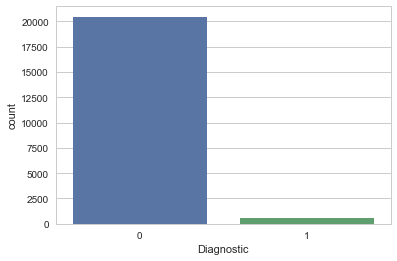
\includegraphics[width=0.6\textwidth]{images/imbalanced_dataset}
\label{records_class}\caption{The number of records by class}
\end{figure} 
% Implementation of the logistic model
\subsubsection{Paramètres du modèle de prédiction.}
 Afin de mettre en place notre modèle de classification basée sur la régression logistique, la librairie sklearn1 de Python \emph{sklearn} library\footnote{https://scikit-learn.org/stable/modules/generated/sklearn.linear\_model.LogisticRegression.html}. Ce package de python définit les paramètres par défaut de la régression logistique, ainsi que des stratégies d'optimisation, pour effectuer correctement la classification binaire en utilisant le meilleur modèle final. Pour les besoins de nos tests, nous avons utilisé les paramètres d'entrée de la régression logistique suivante
 \begin{itemize}
\item \textbf{random\_state}: modélise le l’état initial du générateur de nombres pseudo aléatoires à utiliser lors du mélange des données. Sa valeur est définie à 0 car nous n’avons pas besoin de mélanger les données dans notre expérimentation.
\item \textbf{class\_weight}: c’est le poids associés aux classes. Nous le réglons sur ‘None’, c'est-à-dire que toutes les classes sont censées avoir le poids qui est égale à 1.
\item \textbf{dual}. Il n’est mise en œuvre que pour les problèmes avec une pénalisation l2. Ce paramètre est défini sur Faux car le nombre d’échantillons est supérieur au nombre de fonctionnalités.
\item \textbf{fit\_intercept}: utile si une constante (ou biais) est ajoutée à la fonction de prédiction. Par conséquent, nous avons fixé l’interception d’ajustement à Vrai.
\item \textbf{intercept\_scaling}: ce paramètre, défini sur 1, n'est utile que lorsque le solveur «liblinear» est utilisé et fit_intercept est défini sur Vrai.
\item \textbf{max\_iter}: nombre maximum d'itérations prises pour que les solveurs convergent.
\item \textbf{multi\_class}: si l'option choisie est ovr, alors un problème binaire est correct.
\item \textbf{n\_jobs}: nombre de processeurs cpu utilisés lors de la parallélisation de classes si multi class = "ovr". Ce paramètre est ignoré lorsque le solveur est défini sur “liblinear” que «multiclass» soit spécifié ou non.

\item \textbf{penalty}: ce paramètre est utilisé pour spécifier la norme dans la pénalisation. Nous avons fixé la pénalité à sa valeur par défaut 1/2.
\item \textbf{solver}: il permet de spécifier la stratégie utilisée pour résoudre l'optimisation sous-jacente de notre modèle. Il est fixé à liblinear.
\item \textbf{tol:} tolérance pour le critère d'arrêt définie sur 0.0001.
\item \textbf{verbose}: pour le liblinear solver, définissez verbose sur un nombre positif 
\item \textbf{warm\_start}: lorsqu'il est défini sur True, réutilise la solution de l'appel précédent pour l'adapter à l'initialisation, sinon, effacez la solution précédente. Inutile pour le liblinear solver.
\end{itemize}
Comme la régression logistique effectue un apprentissage supervisé, nous avons utilisé 60\%  du jeu de données pour l’entrainement du modèle et 30\%  du jeu de données  pour  de test.

